\documentclass[11pt,compress,t,notes=noshow, xcolor=table]{beamer}

\usepackage[]{graphicx}\usepackage[]{color}
% maxwidth is the original width if it is less than linewidth
% otherwise use linewidth (to make sure the graphics do not exceed the margin)
\makeatletter
\def\maxwidth{ %
  \ifdim\Gin@nat@width>\linewidth
    \linewidth
  \else
    \Gin@nat@width
  \fi
}
\makeatother

\definecolor{fgcolor}{rgb}{0.345, 0.345, 0.345}
\newcommand{\hlnum}[1]{\textcolor[rgb]{0.686,0.059,0.569}{#1}}%
\newcommand{\hlstr}[1]{\textcolor[rgb]{0.192,0.494,0.8}{#1}}%
\newcommand{\hlcom}[1]{\textcolor[rgb]{0.678,0.584,0.686}{\textit{#1}}}%
\newcommand{\hlopt}[1]{\textcolor[rgb]{0,0,0}{#1}}%
\newcommand{\hlstd}[1]{\textcolor[rgb]{0.345,0.345,0.345}{#1}}%
\newcommand{\hlkwa}[1]{\textcolor[rgb]{0.161,0.373,0.58}{\textbf{#1}}}%
\newcommand{\hlkwb}[1]{\textcolor[rgb]{0.69,0.353,0.396}{#1}}%
\newcommand{\hlkwc}[1]{\textcolor[rgb]{0.333,0.667,0.333}{#1}}%
\newcommand{\hlkwd}[1]{\textcolor[rgb]{0.737,0.353,0.396}{\textbf{#1}}}%
\let\hlipl\hlkwb

\usepackage{framed}
\makeatletter
\newenvironment{kframe}{%
 \def\at@end@of@kframe{}%
 \ifinner\ifhmode%
  \def\at@end@of@kframe{\end{minipage}}%
  \begin{minipage}{\columnwidth}%
 \fi\fi%
 \def\FrameCommand##1{\hskip\@totalleftmargin \hskip-\fboxsep
 \colorbox{shadecolor}{##1}\hskip-\fboxsep
     % There is no \\@totalrightmargin, so:
     \hskip-\linewidth \hskip-\@totalleftmargin \hskip\columnwidth}%
 \MakeFramed {\advance\hsize-\width
   \@totalleftmargin\z@ \linewidth\hsize
   \@setminipage}}%
 {\par\unskip\endMakeFramed%
 \at@end@of@kframe}
\makeatother

\definecolor{shadecolor}{rgb}{.97, .97, .97}
\definecolor{messagecolor}{rgb}{0, 0, 0}
\definecolor{warningcolor}{rgb}{1, 0, 1}
\definecolor{errorcolor}{rgb}{1, 0, 0}
\newenvironment{knitrout}{}{} % an empty environment to be redefined in TeX

\usepackage{alltt}
\newcommand{\SweaveOpts}[1]{}  % do not interfere with LaTeX
\newcommand{\SweaveInput}[1]{} % because they are not real TeX commands
\newcommand{\Sexpr}[1]{}       % will only be parsed by R
\newcommand{\xmark}{\ding{55}}%


\usepackage[english]{babel}
\usepackage[utf8]{inputenc}

\usepackage{dsfont}
\usepackage{verbatim}
\usepackage{amsmath}
\usepackage{amsfonts}
\usepackage{amssymb}
\usepackage{bm}
\usepackage{csquotes}
\usepackage{multirow}
\usepackage{longtable}
\usepackage{booktabs}
\usepackage{enumerate}
\usepackage[absolute,overlay]{textpos}
\usepackage{psfrag}
\usepackage{algorithm}
\usepackage{algpseudocode}
\usepackage{eqnarray}
\usepackage{arydshln}
\usepackage{tabularx}
\usepackage{placeins}
\usepackage{tikz}
\usepackage{setspace}
\usepackage{colortbl}
\usepackage{mathtools}
\usepackage{wrapfig}
\usepackage{bm}
\usepackage{amsmath}
\usepackage{pifont}

\usetikzlibrary{shapes,arrows,automata,positioning,calc,chains,trees, shadows}
\tikzset{
  %Define standard arrow tip
  >=stealth',
  %Define style for boxes
  punkt/.style={
    rectangle,
    rounded corners,
    draw=black, very thick,
    text width=6.5em,
    minimum height=2em,
    text centered},
  % Define arrow style
  pil/.style={
    ->,
    thick,
    shorten <=2pt,
    shorten >=2pt,}
}

\usepackage{subfig}

% Defines macros and environments
\usepackage{../../style/lmu-lecture}


\let\code=\texttt
\let\proglang=\textsf

\setkeys{Gin}{width=0.9\textwidth}

\setbeamertemplate{frametitle}{\expandafter\uppercase\expandafter\insertframetitle}

\usepackage{bbm}
% basic latex stuff
\newcommand{\pkg}[1]{{\fontseries{b}\selectfont #1}} %fontstyle for R packages
\newcommand{\lz}{\vspace{0.5cm}} %vertical space
\newcommand{\dlz}{\vspace{1cm}} %double vertical space
\newcommand{\oneliner}[1] % Oneliner for important statements
{\begin{block}{}\begin{center}\begin{Large}#1\end{Large}\end{center}\end{block}}


%new environments
\newenvironment{vbframe}  %frame with breaks and verbatim
{
 \begin{frame}[containsverbatim,allowframebreaks]
}
{
\end{frame}
}

\newenvironment{vframe}  %frame with verbatim without breaks (to avoid numbering one slided frames)
{
 \begin{frame}[containsverbatim]
}
{
\end{frame}
}

\newenvironment{blocki}[1]   % itemize block
{
 \begin{block}{#1}\begin{itemize}
}
{
\end{itemize}\end{block}
}

\newenvironment{fragileframe}[2]{  %fragile frame with framebreaks
\begin{frame}[allowframebreaks, fragile, environment = fragileframe]
\frametitle{#1}
#2}
{\end{frame}}


\newcommand{\myframe}[2]{  %short for frame with framebreaks
\begin{frame}[allowframebreaks]
\frametitle{#1}
#2
\end{frame}}

\newcommand{\remark}[1]{
  \textbf{Remark:} #1
}


\newenvironment{deleteframe}
{
\begingroup
\usebackgroundtemplate{
\includegraphics[width=\paperwidth,height=\paperheight]{../style/color/red.png}}
 \begin{frame}
}
{
\end{frame}
\endgroup
}
\newenvironment{simplifyframe}
{
\begingroup
\usebackgroundtemplate{
\includegraphics[width=\paperwidth,height=\paperheight]{../style/color/yellow.png}}
 \begin{frame}
}
{
\end{frame}
\endgroup
}\newenvironment{draftframe}
{
\begingroup
\usebackgroundtemplate{
\includegraphics[width=\paperwidth,height=\paperheight]{../style/color/green.jpg}}
 \begin{frame}
}
{
\end{frame}
\endgroup
}
% https://tex.stackexchange.com/a/261480: textcolor that works in mathmode
\makeatletter
\renewcommand*{\@textcolor}[3]{%
  \protect\leavevmode
  \begingroup
    \color#1{#2}#3%
  \endgroup
}
\makeatother





% math spaces
\ifdefined\N                                                                
\renewcommand{\N}{\mathds{N}} % N, naturals
\else \newcommand{\N}{\mathds{N}} \fi 
\newcommand{\Z}{\mathds{Z}} % Z, integers
\newcommand{\Q}{\mathds{Q}} % Q, rationals
\newcommand{\R}{\mathds{R}} % R, reals
\ifdefined\C 
  \renewcommand{\C}{\mathds{C}} % C, complex
\else \newcommand{\C}{\mathds{C}} \fi
\newcommand{\continuous}{\mathcal{C}} % C, space of continuous functions
\newcommand{\M}{\mathcal{M}} % machine numbers
\newcommand{\epsm}{\epsilon_m} % maximum error

% counting / finite sets
\newcommand{\setzo}{\{0, 1\}} % set 0, 1
\newcommand{\setmp}{\{-1, +1\}} % set -1, 1
\newcommand{\unitint}{[0, 1]} % unit interval

% basic math stuff
\newcommand{\xt}{\tilde x} % x tilde
\newcommand{\argmax}{\operatorname{arg\,max}} % argmax
\newcommand{\argmin}{\operatorname{arg\,min}} % argmin
\newcommand{\argminlim}{\mathop{\mathrm{arg\,min}}\limits} % argmax with limits
\newcommand{\argmaxlim}{\mathop{\mathrm{arg\,max}}\limits} % argmin with limits  
\newcommand{\sign}{\operatorname{sign}} % sign, signum
\newcommand{\I}{\mathbb{I}} % I, indicator
\newcommand{\order}{\mathcal{O}} % O, order
\newcommand{\pd}[2]{\frac{\partial{#1}}{\partial #2}} % partial derivative
\newcommand{\floorlr}[1]{\left\lfloor #1 \right\rfloor} % floor
\newcommand{\ceillr}[1]{\left\lceil #1 \right\rceil} % ceiling

% sums and products
\newcommand{\sumin}{\sum\limits_{i=1}^n} % summation from i=1 to n
\newcommand{\sumim}{\sum\limits_{i=1}^m} % summation from i=1 to m
\newcommand{\sumjn}{\sum\limits_{j=1}^n} % summation from j=1 to p
\newcommand{\sumjp}{\sum\limits_{j=1}^p} % summation from j=1 to p
\newcommand{\sumik}{\sum\limits_{i=1}^k} % summation from i=1 to k
\newcommand{\sumkg}{\sum\limits_{k=1}^g} % summation from k=1 to g
\newcommand{\sumjg}{\sum\limits_{j=1}^g} % summation from j=1 to g
\newcommand{\meanin}{\frac{1}{n} \sum\limits_{i=1}^n} % mean from i=1 to n
\newcommand{\meanim}{\frac{1}{m} \sum\limits_{i=1}^m} % mean from i=1 to n
\newcommand{\meankg}{\frac{1}{g} \sum\limits_{k=1}^g} % mean from k=1 to g
\newcommand{\prodin}{\prod\limits_{i=1}^n} % product from i=1 to n
\newcommand{\prodkg}{\prod\limits_{k=1}^g} % product from k=1 to g
\newcommand{\prodjp}{\prod\limits_{j=1}^p} % product from j=1 to p

% linear algebra
\newcommand{\one}{\boldsymbol{1}} % 1, unitvector
\newcommand{\zero}{\mathbf{0}} % 0-vector
\newcommand{\id}{\boldsymbol{I}} % I, identity
\newcommand{\diag}{\operatorname{diag}} % diag, diagonal
\newcommand{\trace}{\operatorname{tr}} % tr, trace
\newcommand{\spn}{\operatorname{span}} % span
\newcommand{\scp}[2]{\left\langle #1, #2 \right\rangle} % <.,.>, scalarproduct
\newcommand{\mat}[1]{\begin{pmatrix} #1 \end{pmatrix}} % short pmatrix command
\newcommand{\Amat}{\mathbf{A}} % matrix A
\newcommand{\Deltab}{\mathbf{\Delta}} % error term for vectors

% basic probability + stats
\renewcommand{\P}{\mathds{P}} % P, probability
\newcommand{\E}{\mathds{E}} % E, expectation
\newcommand{\var}{\mathsf{Var}} % Var, variance
\newcommand{\cov}{\mathsf{Cov}} % Cov, covariance
\newcommand{\corr}{\mathsf{Corr}} % Corr, correlation
\newcommand{\normal}{\mathcal{N}} % N of the normal distribution
\newcommand{\iid}{\overset{i.i.d}{\sim}} % dist with i.i.d superscript
\newcommand{\distas}[1]{\overset{#1}{\sim}} % ... is distributed as ...

% machine learning
\newcommand{\Xspace}{\mathcal{X}} % X, input space
\newcommand{\Yspace}{\mathcal{Y}} % Y, output space
\newcommand{\nset}{\{1, \ldots, n\}} % set from 1 to n
\newcommand{\pset}{\{1, \ldots, p\}} % set from 1 to p
\newcommand{\gset}{\{1, \ldots, g\}} % set from 1 to g
\newcommand{\Pxy}{\mathbb{P}_{xy}} % P_xy
\newcommand{\Exy}{\mathbb{E}_{xy}} % E_xy: Expectation over random variables xy
\newcommand{\xv}{\mathbf{x}} % vector x (bold)
\newcommand{\xtil}{\tilde{\mathbf{x}}} % vector x-tilde (bold)
\newcommand{\yv}{\mathbf{y}} % vector y (bold)
\newcommand{\xy}{(\xv, y)} % observation (x, y)
\newcommand{\xvec}{\left(x_1, \ldots, x_p\right)^\top} % (x1, ..., xp) 
\newcommand{\Xmat}{\mathbf{X}} % Design matrix
\newcommand{\allDatasets}{\mathds{D}} % The set of all datasets
\newcommand{\allDatasetsn}{\mathds{D}_n}  % The set of all datasets of size n 
\newcommand{\D}{\mathcal{D}} % D, data
\newcommand{\Dn}{\D_n} % D_n, data of size n
\newcommand{\Dtrain}{\mathcal{D}_{\text{train}}} % D_train, training set
\newcommand{\Dtest}{\mathcal{D}_{\text{test}}} % D_test, test set
\newcommand{\xyi}[1][i]{\left(\xv^{(#1)}, y^{(#1)}\right)} % (x^i, y^i), i-th observation
\newcommand{\Dset}{\left( \xyi[1], \ldots, \xyi[n]\right)} % {(x1,y1)), ..., (xn,yn)}, data
\newcommand{\defAllDatasetsn}{(\Xspace \times \Yspace)^n} % Def. of the set of all datasets of size n 
\newcommand{\defAllDatasets}{\bigcup_{n \in \N}(\Xspace \times \Yspace)^n} % Def. of the set of all datasets 
\newcommand{\xdat}{\left\{ \xv^{(1)}, \ldots, \xv^{(n)}\right\}} % {x1, ..., xn}, input data
\newcommand{\yvec}{\left(y^{(1)}, \hdots, y^{(n)}\right)^\top} % (y1, ..., yn), vector of outcomes
\renewcommand{\xi}[1][i]{\xv^{(#1)}} % x^i, i-th observed value of x
\newcommand{\yi}[1][i]{y^{(#1)}} % y^i, i-th observed value of y 
\newcommand{\xivec}{\left(x^{(i)}_1, \ldots, x^{(i)}_p\right)^\top} % (x1^i, ..., xp^i), i-th observation vector
\newcommand{\xj}{\xv_j} % x_j, j-th feature
\newcommand{\xjvec}{\left(x^{(1)}_j, \ldots, x^{(n)}_j\right)^\top} % (x^1_j, ..., x^n_j), j-th feature vector
\newcommand{\phiv}{\mathbf{\phi}} % Basis transformation function phi
\newcommand{\phixi}{\mathbf{\phi}^{(i)}} % Basis transformation of xi: phi^i := phi(xi)

%%%%%% ml - models general
\newcommand{\lamv}{\bm{\lambda}} % lambda vector, hyperconfiguration vector
\newcommand{\Lam}{\bm{\Lambda}}	 % Lambda, space of all hpos
% Inducer / Inducing algorithm
\newcommand{\preimageInducer}{\left(\defAllDatasets\right)\times\Lam} % Set of all datasets times the hyperparameter space
\newcommand{\preimageInducerShort}{\allDatasets\times\Lam} % Set of all datasets times the hyperparameter space
% Inducer / Inducing algorithm
\newcommand{\ind}{\mathcal{I}} % Inducer, inducing algorithm, learning algorithm 

% continuous prediction function f
\newcommand{\ftrue}{f_{\text{true}}}  % True underlying function (if a statistical model is assumed)
\newcommand{\ftruex}{\ftrue(\xv)} % True underlying function (if a statistical model is assumed)
\newcommand{\fx}{f(\xv)} % f(x), continuous prediction function
\newcommand{\fdomains}{f: \Xspace \rightarrow \R^g} % f with domain and co-domain
\newcommand{\Hspace}{\mathcal{H}} % hypothesis space where f is from
\newcommand{\fbayes}{f^{\ast}} % Bayes-optimal model
\newcommand{\fxbayes}{f^{\ast}(\xv)} % Bayes-optimal model
\newcommand{\fkx}[1][k]{f_{#1}(\xv)} % f_j(x), discriminant component function
\newcommand{\fh}{\hat{f}} % f hat, estimated prediction function
\newcommand{\fxh}{\fh(\xv)} % fhat(x)
\newcommand{\fxt}{f(\xv ~|~ \thetab)} % f(x | theta)
\newcommand{\fxi}{f\left(\xv^{(i)}\right)} % f(x^(i))
\newcommand{\fxih}{\hat{f}\left(\xv^{(i)}\right)} % f(x^(i))
\newcommand{\fxit}{f\left(\xv^{(i)} ~|~ \thetab\right)} % f(x^(i) | theta)
\newcommand{\fhD}{\fh_{\D}} % fhat_D, estimate of f based on D
\newcommand{\fhDtrain}{\fh_{\Dtrain}} % fhat_Dtrain, estimate of f based on D
\newcommand{\fhDnlam}{\fh_{\Dn, \lamv}} %model learned on Dn with hp lambda
\newcommand{\fhDlam}{\fh_{\D, \lamv}} %model learned on D with hp lambda
\newcommand{\fhDnlams}{\fh_{\Dn, \lamv^\ast}} %model learned on Dn with optimal hp lambda 
\newcommand{\fhDlams}{\fh_{\D, \lamv^\ast}} %model learned on D with optimal hp lambda 

% discrete prediction function h
\newcommand{\hx}{h(\xv)} % h(x), discrete prediction function
\newcommand{\hh}{\hat{h}} % h hat
\newcommand{\hxh}{\hat{h}(\xv)} % hhat(x)
\newcommand{\hxt}{h(\xv | \thetab)} % h(x | theta)
\newcommand{\hxi}{h\left(\xi\right)} % h(x^(i))
\newcommand{\hxit}{h\left(\xi ~|~ \thetab\right)} % h(x^(i) | theta)
\newcommand{\hbayes}{h^{\ast}} % Bayes-optimal classification model
\newcommand{\hxbayes}{h^{\ast}(\xv)} % Bayes-optimal classification model

% yhat
\newcommand{\yh}{\hat{y}} % yhat for prediction of target
\newcommand{\yih}{\hat{y}^{(i)}} % yhat^(i) for prediction of ith targiet
\newcommand{\resi}{\yi- \yih}

% theta
\newcommand{\thetah}{\hat{\theta}} % theta hat
\newcommand{\thetab}{\bm{\theta}} % theta vector
\newcommand{\thetabh}{\bm{\hat\theta}} % theta vector hat
\newcommand{\thetat}[1][t]{\thetab^{[#1]}} % theta^[t] in optimization
\newcommand{\thetatn}[1][t]{\thetab^{[#1 +1]}} % theta^[t+1] in optimization
\newcommand{\thetahDnlam}{\thetabh_{\Dn, \lamv}} %theta learned on Dn with hp lambda
\newcommand{\thetahDlam}{\thetabh_{\D, \lamv}} %theta learned on D with hp lambda
\newcommand{\mint}{\min_{\thetab \in \Theta}} % min problem theta
\newcommand{\argmint}{\argmin_{\thetab \in \Theta}} % argmin theta

% densities + probabilities
% pdf of x 
\newcommand{\pdf}{p} % p
\newcommand{\pdfx}{p(\xv)} % p(x)
\newcommand{\pixt}{\pi(\xv~|~ \thetab)} % pi(x|theta), pdf of x given theta
\newcommand{\pixit}{\pi\left(\xi ~|~ \thetab\right)} % pi(x^i|theta), pdf of x given theta
\newcommand{\pixii}{\pi\left(\xi\right)} % pi(x^i), pdf of i-th x 

% pdf of (x, y)
\newcommand{\pdfxy}{p(\xv,y)} % p(x, y)
\newcommand{\pdfxyt}{p(\xv, y ~|~ \thetab)} % p(x, y | theta)
\newcommand{\pdfxyit}{p\left(\xi, \yi ~|~ \thetab\right)} % p(x^(i), y^(i) | theta)

% pdf of x given y
\newcommand{\pdfxyk}[1][k]{p(\xv | y= #1)} % p(x | y = k)
\newcommand{\lpdfxyk}[1][k]{\log p(\xv | y= #1)} % log p(x | y = k)
\newcommand{\pdfxiyk}[1][k]{p\left(\xi | y= #1 \right)} % p(x^i | y = k)

% prior probabilities
\newcommand{\pik}[1][k]{\pi_{#1}} % pi_k, prior
\newcommand{\lpik}[1][k]{\log \pi_{#1}} % log pi_k, log of the prior
\newcommand{\pit}{\pi(\thetab)} % Prior probability of parameter theta

% posterior probabilities
\newcommand{\post}{\P(y = 1 ~|~ \xv)} % P(y = 1 | x), post. prob for y=1
\newcommand{\postk}[1][k]{\P(y = #1 ~|~ \xv)} % P(y = k | y), post. prob for y=k
\newcommand{\pidomains}{\pi: \Xspace \rightarrow \unitint} % pi with domain and co-domain
\newcommand{\pibayes}{\pi^{\ast}} % Bayes-optimal classification model
\newcommand{\pixbayes}{\pi^{\ast}(\xv)} % Bayes-optimal classification model
\newcommand{\pix}{\pi(\xv)} % pi(x), P(y = 1 | x)
\newcommand{\pikx}[1][k]{\pi_{#1}(\xv)} % pi_k(x), P(y = k | x)
\newcommand{\pikxt}[1][k]{\pi_{#1}(\xv ~|~ \thetab)} % pi_k(x | theta), P(y = k | x, theta)
\newcommand{\pixh}{\hat \pi(\xv)} % pi(x) hat, P(y = 1 | x) hat
\newcommand{\pikxh}[1][k]{\hat \pi_{#1}(\xv)} % pi_k(x) hat, P(y = k | x) hat
\newcommand{\pixih}{\hat \pi(\xi)} % pi(x^(i)) with hat
\newcommand{\pikxih}[1][k]{\hat \pi_{#1}(\xi)} % pi_k(x^(i)) with hat
\newcommand{\pdfygxt}{p(y ~|~\xv, \thetab)} % p(y | x, theta)
\newcommand{\pdfyigxit}{p\left(\yi ~|~\xi, \thetab\right)} % p(y^i |x^i, theta)
\newcommand{\lpdfygxt}{\log \pdfygxt } % log p(y | x, theta)
\newcommand{\lpdfyigxit}{\log \pdfyigxit} % log p(y^i |x^i, theta)

% probababilistic
\newcommand{\bayesrulek}[1][k]{\frac{\P(\xv | y= #1) \P(y= #1)}{\P(\xv)}} % Bayes rule
\newcommand{\muk}{\bm{\mu_k}} % mean vector of class-k Gaussian (discr analysis) 

% residual and margin
\newcommand{\eps}{\epsilon} % residual, stochastic
\newcommand{\epsi}{\epsilon^{(i)}} % epsilon^i, residual, stochastic
\newcommand{\epsh}{\hat{\epsilon}} % residual, estimated
\newcommand{\yf}{y \fx} % y f(x), margin
\newcommand{\yfi}{\yi \fxi} % y^i f(x^i), margin
\newcommand{\Sigmah}{\hat \Sigma} % estimated covariance matrix
\newcommand{\Sigmahj}{\hat \Sigma_j} % estimated covariance matrix for the j-th class

% ml - loss, risk, likelihood
\newcommand{\Lyf}{L\left(y, f\right)} % L(y, f), loss function
\newcommand{\Lxy}{L\left(y, \fx\right)} % L(y, f(x)), loss function
\newcommand{\Lxyi}{L\left(\yi, \fxi\right)} % loss of observation
\newcommand{\Lxyt}{L\left(y, \fxt\right)} % loss with f parameterized
\newcommand{\Lxyit}{L\left(\yi, \fxit\right)} % loss of observation with f parameterized
\newcommand{\Lxym}{L\left(\yi, f\left(\bm{\tilde{x}}^{(i)} ~|~ \thetab\right)\right)} % loss of observation with f parameterized
\newcommand{\Lpixy}{L\left(y, \pix\right)} % loss in classification
\newcommand{\Lpixyi}{L\left(\yi, \pixii\right)} % loss of observation in classification
\newcommand{\Lpixyt}{L\left(y, \pixt\right)} % loss with pi parameterized
\newcommand{\Lpixyit}{L\left(\yi, \pixit\right)} % loss of observation with pi parameterized
\newcommand{\Lhxy}{L\left(y, \hx\right)} % L(y, h(x)), loss function on discrete classes
\newcommand{\Lr}{L\left(r\right)} % L(r), loss defined on residual (reg) / margin (classif)
\newcommand{\lone}{|y - \fx|} % L1 loss
\newcommand{\ltwo}{\left(y - \fx\right)^2} % L2 loss
\newcommand{\lbernoullimp}{\ln(1 + \exp(-y \cdot \fx))} % Bernoulli loss for -1, +1 encoding
\newcommand{\lbernoullizo}{- y \cdot \fx + \log(1 + \exp(\fx))} % Bernoulli loss for 0, 1 encoding
\newcommand{\lcrossent}{- y \log \left(\pix\right) - (1 - y) \log \left(1 - \pix\right)} % cross-entropy loss
\newcommand{\lbrier}{\left(\pix - y \right)^2} % Brier score
\newcommand{\risk}{\mathcal{R}} % R, risk
\newcommand{\riskbayes}{\mathcal{R}^\ast}
\newcommand{\riskf}{\risk(f)} % R(f), risk
\newcommand{\riskdef}{\E_{y|\xv}\left(\Lxy \right)} % risk def (expected loss)
\newcommand{\riskt}{\mathcal{R}(\thetab)} % R(theta), risk
\newcommand{\riske}{\mathcal{R}_{\text{emp}}} % R_emp, empirical risk w/o factor 1 / n
\newcommand{\riskeb}{\bar{\mathcal{R}}_{\text{emp}}} % R_emp, empirical risk w/ factor 1 / n
\newcommand{\riskef}{\riske(f)} % R_emp(f)
\newcommand{\risket}{\mathcal{R}_{\text{emp}}(\thetab)} % R_emp(theta)
\newcommand{\riskr}{\mathcal{R}_{\text{reg}}} % R_reg, regularized risk
\newcommand{\riskrt}{\mathcal{R}_{\text{reg}}(\thetab)} % R_reg(theta)
\newcommand{\riskrf}{\riskr(f)} % R_reg(f)
\newcommand{\riskrth}{\hat{\mathcal{R}}_{\text{reg}}(\thetab)} % hat R_reg(theta)
\newcommand{\risketh}{\hat{\mathcal{R}}_{\text{emp}}(\thetab)} % hat R_emp(theta)
\newcommand{\LL}{\mathcal{L}} % L, likelihood
\newcommand{\LLt}{\mathcal{L}(\thetab)} % L(theta), likelihood
\newcommand{\LLtx}{\mathcal{L}(\thetab | \xv)} % L(theta|x), likelihood
\newcommand{\logl}{\ell} % l, log-likelihood
\newcommand{\loglt}{\logl(\thetab)} % l(theta), log-likelihood
\newcommand{\logltx}{\logl(\thetab | \xv)} % l(theta|x), log-likelihood
\newcommand{\errtrain}{\text{err}_{\text{train}}} % training error
\newcommand{\errtest}{\text{err}_{\text{test}}} % test error
\newcommand{\errexp}{\overline{\text{err}_{\text{test}}}} % avg training error

% lm
\newcommand{\thx}{\thetab^\top \xv} % linear model
\newcommand{\olsest}{(\Xmat^\top \Xmat)^{-1} \Xmat^\top \yv} % OLS estimator in LM 


\newcommand{\sens}{\mathbf{A}} % vector x (bold)
\newcommand{\ba}{\mathbf{a}}
\newcommand{\batilde}{\tilde{\mathbf{a}}}
\newcommand{\Px}{\mathbb{P}_{x}} % P_x
\newcommand{\Pxj}{\mathbb{P}_{x_j}} % P_{x_j}
\newcommand{\indep}{\perp \!\!\! \perp} % independence symbol
% ml - ROC
\newcommand{\np}{n_{+}} % no. of positive instances
\newcommand{\nn}{n_{-}} % no. of negative instances
\newcommand{\rn}{\pi_{-}} % proportion negative instances
\newcommand{\rp}{\pi_{+}} % proportion negative instances
% true/false pos/neg:
\newcommand{\tp}{\# \text{TP}} % true pos
\newcommand{\fap}{\# \text{FP}} % false pos (fp taken for partial derivs)
\newcommand{\tn}{\# \text{TN}} % true neg
\newcommand{\fan}{\# \text{FN}} % false neg

\newcommand{\Tspace}{\mathcal{T}}
\newcommand{\tv}{\mathbf{t}}
\newcommand{\tj}{\mathbf{t}_j}

\usepackage{multicol}
\usepackage{color,colortbl} 
\definecolor{putblue}{RGB}{0,0,124}
\definecolor{putred}{RGB}{204,33,69}

\newcommand{\titlefigure}{figure/fmeasure}
\newcommand{\learninggoals}{
  \item Get to know loss functions for multi-target prediction problems
  \item Know the Bayes predictor for Hamming loss and subset $0/1$ loss
  \item Understand the difference between macro-, micro-, and instance-wise-losses 
}

\title{Advanced Machine Learning}
\date{}

\begin{document}

\lecturechapter{Loss Functions for Multi-Target Prediction}
\lecture{Advanced Machine Learning}



\sloppy


\begin{frame}
	\frametitle{Multivariate Loss Functions}
	\begin{itemize}
%		
		\small
%		
		\item In multi-target prediction we want to the following: For a feature vector $\xv$, predict a vector of scores $\yv = (y_1, y_2, \ldots, y_m)^\top$ by means of a function (hypothesis) $f$:
		$$
		\xv = (x_1,x_2,\ldots,x_p)^\top \quad \xrightarrow{~~\fx~~} \quad \yh = ( \hat{y}_1, \hat{y}_2, \ldots, \hat{y}_m)^\top
		$$
%		
		\item If we want to follow the machine learning paradigm based on loss minimization, we need a \emph{multivariate loss functions} 
		$$
		\ell: \, \Yspace^m \times \Yspace^m \rightarrow \mathbb{R}.
		$$  
		Compared to single-target prediction,  a broad spectrum of such multivariate loss functions	is conceivable. 
%		
		\item In case we have an appropriate multivariate loss function $\ell$, we want to find a (Bayes) predictor $\fbayes$ that minimizes expected loss with regard to $\ell:$
%		
		\begin{eqnarray*}
			\fbayes &=& \argmin_{f: \Xspace \to \Yspace^m} \risk_\ell \left(f\right) = \argmin_{f: \Xspace \to \Yspace^m}\Exy\left[ \ell(y,\fx) \right]\\ &=&  \argmin_{f: \Xspace \to \Yspace^m }\int \ell(y,\fx) \text{d}\Pxy. 
		\end{eqnarray*}
%				
%		\item Can we achieve this goal through simple reduction, i.e., by training one model for each target independently? Or can we do better with more sophisticated methods?  
%		
%		\item There are \emph{two views:} the individual target and joint target view.
%
	\end{itemize}
	
\end{frame}




\begin{frame}
	\frametitle{Examples of MTP loss functions}
	\begin{itemize}
		
		\small 
		\item \emph{Squared error loss} (typically used in multivariate regression):
		$$
		\ell(\yv, \yh) = \sum_{j=1}^m (y_j - \hat{y}_j)^2 \, ,
		$$
		where $\yv , \yh \in \mathbb{R}^m$.
		
		
		\medskip
		
		
		%		
		%		\item \emph{F-measure}:
		%		$$
		%		F(\mathbf{Y}, \hat{\mathbf{Y}}) = \frac{2 \sum_{i=1}^K y_i \hat{y}_i}{\sum_{i=1}^K y_i + \sum_{i=1}^K \hat{y}_i} \, ,
		%		$$
		%		where $\mathbf{Y} = (y_1, \ldots , y_K) \in \{ 0,1 \}^K$ and $\hat{\mathbf{Y}} = (\hat{y}_1, \ldots , \hat{y}_K) \in \{ 0,1 \}^K$. Can be used in macro- and micro-averaging, but also instance-wise. 
		%		
		
		
		\item The \emph{Hamming loss} averages over mistakes on individual scores:    
		$$
		\displaystyle \ell_H(\yv, \hat{y}) = \frac{1}{m}  \, \sum_{j=1}^m \, \mathds{1}_{[y_j \neq  \hat y_j ]}
		$$
		
		\item The \emph{subset 0/1 loss} simply checks for entire correctness:  
		\begin{align*}
			\displaystyle \ell_{0/1}(\yv, \hat{y}) & = \mathds{1}_{[ \yv \ne \hat{y} ]}  =  \max_j \, \mathds{1}_{[y_j \neq  \hat y_j]}
		\end{align*}
		
		
	\end{itemize}
\end{frame}



\begin{frame}
	\frametitle{Hamming vs.\ subset 0/1 loss}
	\begin{itemize}
		\item The risk minimizer for the Hamming loss is the  \emph{marginal mode}:
		$$
		f_j^*(\xv) = \arg \max_{y_j \in \{0,1\}} \Pr( y_j  ~|~ \xv )\,, \quad j = 1,\ldots,m ,
		$$
		%\item 
		while for the subset 0/1 loss it is the \emph{joint mode}:
		$$
		\mathbf{f}^*(\xv) = \arg \max_{\yv \in \mathcal{Y}^m} \Pr(\yv ~|~ \xv) \,.
		$$
		\item Marginal mode vs. joint mode:\\[6pt]
		\begin{center}
			\begin{tabular}{@{}cc@{}}
				\toprule
				$\yv$ & $\Pr(\yv)$ \\
				\hline
				$0~0~0~0$ & $0.30$ \\
				$0~1~1~1$ & $0.17$ \\
				$1~0~1~1$ & $0.18$ \\
				$1~1~0~1$ & $0.17$ \\
				$1~1~1~0$ & $0.18$ \\
				\toprule
			\end{tabular}
			$\qquad$
			\footnotesize{
				\begin{tabular}{lr}
					Marginal mode: & $1~1~1~1$ \\
					Joint mode: & $0~0~0~0$ \\
				\end{tabular}
			}
		\end{center}
	\end{itemize}
\end{frame}



%\begin{frame}
%	\frametitle{The individual target view}
%	
%	\begin{itemize} 
%		\item How can we improve the predictive accuracy of a single label \yv exploiting information about other labels?
%		\item Goal: predict a value of $y_i$ using $\xv$ and any available information on other targets $y_j$.
%		\item The problem is usually defined through univariate losses $\ell_i(y_i, \hat{y}_i)$.
%		%\item The problem is usually decomposable over the targets.
%		\item  Domain of $y_i$ is either continuous or nominal.
%		\item  Independent models vs.\ regularized (shrunken) models.
%%		\item James-Stein paradox (to be discussed later).
%		
%	\end{itemize}
%	
%\end{frame}
%
%
%
%\begin{frame}
%	\frametitle{The joint target view}
%	
%	\begin{itemize}
%		\item The problem is defined through multivariate losses $\ell(\yv, \yh)$.
%		%\item What are examples of such loss functions ?
%		\item Is reduction to single-target prediction (decomposition over targets) still possible, and even if so, can we improve over such strategies \yv using more expressive models?
%		%\item What are the relations between the losses?
%		%\item Goal: predict a vector $\yv$ using $\xv$.
%		\item Important: \emph{Structure of loss} $\ell(\cdot, \cdot)$, possible \emph{dependencies between targets}, multivariate distribution of $\yv$.
%		
%		%\item The problem might not be easily decomposable over the targets.
%		%\item Domain of $\yv$ is usually finite, but contains a large number of elements.
%		%\item Independent models vs.\ more expressive models.
%		%\item Loss function perspective.
%		
%	\end{itemize}
%\end{frame}


\begin{frame}
	\frametitle{Multivariate loss functions}
	\small
	\begin{itemize}
%		
%		\item 
%
		\item A loss $L$ (on test data) is decomposable over examples if it can be written in the form
		$$
		L = \sum_{i=1}^n \ell(\yv^{(i)}, f(\xi)) 
		%\quad \text{vs.} \quad L \ne \sum_{i=1}^n \ell(\yv^{(i)}, f(\xi)) 
		\, ,
		$$
		i.e., as a sum of losses over all (test) examples. 
		
		
		\item A multivariate loss $\ell$ is decomposable over targets if it can be written as
		$$
		\ell(\yv, \fx) = \sum_{j=1}^m \ell_j(y_j, f_j(\xv)) 
		%\quad \text{vs.} \quad \ell(\yv, \fx) \ne \sum_{i=1}^m \ell(y_i, h_i(\xv))
		$$
		with suitable single-target losses $\ell_j$. 
		
%		

		\begin{minipage}{0.45\textwidth}
%			
			\item  In general, we distinguish between three categories of losses: macro-, micro-, and instance-wise-losses. 
%			
		\end{minipage}
%	
		\begin{minipage}{0.45\textwidth}
			\begin{center}
				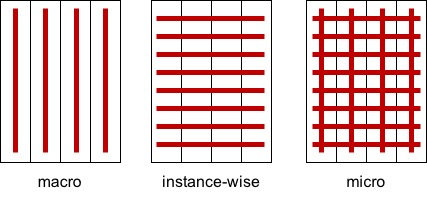
\includegraphics[width=0.9\textwidth]{figure/fmeasure}
			\end{center}
		\end{minipage}
%		
	\end{itemize}
%
\end{frame}






\begin{frame}
	\frametitle{Macro- and micro-Losses}
	
	\begin{itemize}
		\item<1-> Macro-losses: The overall loss corresponds to aggregating the losses over the targets.
		
		\begin{center}
			\begin{tabular}{|c|c|c|c|}
				\multicolumn{4}{c}{True scores} \\
				\hline
				{\only<2>{\color{putred}}$y_{11}$} & {\only<3>{\color{putred}}$y_{12}$} & {\only<4>{\color{putred}}$y_{13}$} & {\only<5>{\color{putred}}$y_{14}$} \\
				{\only<2>{\color{putred}}$y_{21}$} & {\only<3>{\color{putred}}$y_{22}$} & {\only<4>{\color{putred}}$y_{23}$} & {\only<5>{\color{putred}}$y_{24}$} \\
				{\only<2>{\color{putred}}$y_{31}$} & {\only<3>{\color{putred}}$y_{32}$} & {\only<4>{\color{putred}}$y_{33}$} & {\only<5>{\color{putred}}$y_{34}$} \\
				{\only<2>{\color{putred}}$y_{41}$} & {\only<3>{\color{putred}}$y_{42}$} & {\only<4>{\color{putred}}$y_{43}$} & {\only<5>{\color{putred}}$y_{44}$} \\
				{\only<2>{\color{putred}}$y_{51}$} & {\only<3>{\color{putred}}$y_{52}$} & {\only<4>{\color{putred}}$y_{53}$} & {\only<5>{\color{putred}}$y_{54}$} \\
				{\only<2>{\color{putred}}$y_{61}$} & {\only<3>{\color{putred}}$y_{62}$} & {\only<4>{\color{putred}}$y_{63}$} & {\only<5>{\color{putred}}$y_{64}$} \\
				\hline
			\end{tabular}
			$\quad$
			\begin{tabular}{|c|c|c|c|}
				\multicolumn{4}{c}{Predicted scores} \\
				\hline
				{\only<2>{\color{putred}}$\hat{y}_{11}$} & {\only<3>{\color{putred}}$\hat{y}_{12}$} & {\only<4>{\color{putred}}$\hat{y}_{13}$} & {\only<5>{\color{putred}}$\hat{y}_{14}$} \\
				{\only<2>{\color{putred}}$\hat{y}_{21}$} & {\only<3>{\color{putred}}$\hat{y}_{22}$} & {\only<4>{\color{putred}}$\hat{y}_{23}$} & {\only<5>{\color{putred}}$\hat{y}_{24}$} \\
				{\only<2>{\color{putred}}$\hat{y}_{31}$} & {\only<3>{\color{putred}}$\hat{y}_{32}$} & {\only<4>{\color{putred}}$\hat{y}_{33}$} & {\only<5>{\color{putred}}$\hat{y}_{34}$} \\
				{\only<2>{\color{putred}}$\hat{y}_{41}$} & {\only<3>{\color{putred}}$\hat{y}_{42}$} & {\only<4>{\color{putred}}$\hat{y}_{43}$} & {\only<5>{\color{putred}}$\hat{y}_{44}$} \\
				{\only<2>{\color{putred}}$\hat{y}_{51}$} & {\only<3>{\color{putred}}$\hat{y}_{52}$} & {\only<4>{\color{putred}}$\hat{y}_{53}$} & {\only<5>{\color{putred}}$\hat{y}_{54}$} \\
				{\only<2>{\color{putred}}$\hat{y}_{61}$} & {\only<3>{\color{putred}}$\hat{y}_{62}$} & {\only<4>{\color{putred}}$\hat{y}_{63}$} & {\only<5>{\color{putred}}$\hat{y}_{64}$} \\
				\hline
			\end{tabular}
		\end{center}
	\lz
	\item Example: Averaging the target losses.
	$$
	L = \frac{1}{4} \left( {\only<2>{\color{putred}}L_1} + {\only<3>{\color{putred}}L_2} + {\only<4>{\color{putred}}L_3} + {\only<5>{\color{putred}}L_4} \right)
	$$
	\end{itemize}
	

	
\end{frame}




\begin{frame}
	\frametitle{Macro- and micro-Losses}
	
	\begin{itemize}
		\item<1-> Micro-losses: The overall loss corresponds to aggregating the pointwise losses over the targets and the instances.
		
		\begin{center}
			\begin{tabular}{|c|c|c|c|}
				\multicolumn{4}{c}{True scores} \\
				\hline
				\color{putred}$y_{11}$ & \color{putred}$y_{12}$ & \color{putred}$y_{13}$ & \color{putred}$y_{14}$ \\
				\color{putred}$y_{21}$ & \color{putred}$y_{22}$ & \color{putred}$y_{23}$ & \color{putred}$y_{24}$ \\
				\color{putred}$y_{31}$ & \color{putred}$y_{32}$ & \color{putred}$y_{33}$ & \color{putred}$y_{34}$ \\
				\color{putred}$y_{41}$ & \color{putred}$y_{42}$ & \color{putred}$y_{43}$ & \color{putred}$y_{44}$ \\
				\color{putred}$y_{51}$ & \color{putred}$y_{52}$ & \color{putred}$y_{53}$ & \color{putred}$y_{54}$ \\
				\color{putred}$y_{61}$ & \color{putred}$y_{62}$ & \color{putred}$y_{63}$ & \color{putred}$y_{64}$ \\
				\hline
			\end{tabular}
			$\quad$
			\begin{tabular}{|c|c|c|c|}
				\multicolumn{4}{c}{Predicted scores} \\
				\hline
				\color{putred}$\hat{y}_{11}$ & \color{putred}$\hat{y}_{12}$ & \color{putred}$\hat{y}_{13}$ & \color{putred}$\hat{y}_{14}$ \\
				\color{putred}$\hat{y}_{21}$ & \color{putred}$\hat{y}_{22}$ & \color{putred}$\hat{y}_{23}$ & \color{putred}$\hat{y}_{24}$ \\
				\color{putred}$\hat{y}_{31}$ & \color{putred}$\hat{y}_{32}$ & \color{putred}$\hat{y}_{33}$ & \color{putred}$\hat{y}_{34}$ \\
				\color{putred}$\hat{y}_{41}$ & \color{putred}$\hat{y}_{42}$ & \color{putred}$\hat{y}_{43}$ & \color{putred}$\hat{y}_{44}$ \\
				\color{putred}$\hat{y}_{51}$ & \color{putred}$\hat{y}_{52}$ & \color{putred}$\hat{y}_{53}$ & \color{putred}$\hat{y}_{54}$ \\
				\color{putred}$\hat{y}_{61}$ & \color{putred}$\hat{y}_{62}$ & \color{putred}$\hat{y}_{63}$ & \color{putred}$\hat{y}_{64}$ \\
				\hline
			\end{tabular}
		\end{center}
	\lz
	\item Thus, we have	
	$$
	L =  \sum_{i,j} \ell(y_{ij} , \hat{y}_{ij}),
	$$
	where $\ell: \Yspace \times \Yspace \to \R$ in this case.
%	
	\end{itemize}

\end{frame}


\begin{frame}
	\frametitle{Macro- and micro-Losses}
	
	\begin{itemize}
		\item<1-> Micro-losses: The overall loss corresponds to averaging the pointwise losses over the targets and the instances.
		
		\begin{center}
			\begin{tabular}{|c|c|c|c|}
				\multicolumn{4}{c}{True scores} \\
				\hline
				\color{putred}$y_{11}$ & \color{putred}$y_{12}$ &   & \color{putred}$y_{14}$ \\
				\color{putred}$y_{21}$ &   & \color{putred}$y_{23}$ & \color{putred}$y_{24}$ \\
				\color{putred}$y_{31}$ & \color{putred}$y_{32}$ & \color{putred}$y_{33}$ & \color{putred}$y_{34}$ \\
				\color{putred}$y_{41}$ &   & \color{putred}$y_{43}$ & \color{putred}$y_{44}$ \\
				\color{putred}$y_{51}$ & \color{putred}$y_{52}$ & \color{putred}$y_{53}$ & \color{putred}$y_{54}$ \\
				& \color{putred}$y_{62}$ & \color{putred}$y_{63}$ &   \\
				\hline
			\end{tabular}
			$\quad$
			\begin{tabular}{|c|c|c|c|}
				\multicolumn{4}{c}{Predicted scores} \\
				\hline
				\color{putred}$\hat{y}_{11}$ & \color{putred}$\hat{y}_{12}$ &   & \color{putred}$\hat{y}_{14}$ \\
				\color{putred}$\hat{y}_{21}$ &   & \color{putred}$\hat{y}_{23}$ & \color{putred}$\hat{y}_{24}$ \\
				\color{putred}$\hat{y}_{31}$ & \color{putred}$\hat{y}_{32}$ & \color{putred}$\hat{y}_{33}$ & \color{putred}$\hat{y}_{34}$ \\
				\color{putred}$\hat{y}_{41}$ &   & \color{putred}$\hat{y}_{43}$ & \color{putred}$\hat{y}_{44}$ \\
				\color{putred}$\hat{y}_{51}$ & \color{putred}$\hat{y}_{52}$ & \color{putred}$\hat{y}_{53}$ & \color{putred}$\hat{y}_{54}$ \\
				& \color{putred}$\hat{y}_{62}$ & \color{putred}$\hat{y}_{63}$ &   \\
				\hline
			\end{tabular}
		\end{center}	
	\lz
	\item Thus, we have	
		$$
	L =  \sum_{i,j} \ell(y_{ij} , \hat{y}_{ij}),
	$$
	where $\ell: \Yspace \times \Yspace \to \R$ in this case.
%	
	\item 	
		Can be used also for cases with missing entries.
	\end{itemize}
 

	
\end{frame}




\begin{frame}
	\frametitle{Instance-wise losses}
	
	\begin{itemize}
		\item<1-> Instance-wise losses: Aggregating the losses over the instances.
		
		\begin{center}
			\begin{tabular}{|c|c|c|c|}
				\multicolumn{4}{c}{True scores} \\
				\hline
				{\only<2>{\color{putred}}$y_{11}$} & {\only<2>{\color{putred}}$y_{12}$} & {\only<2>{\color{putred}}$y_{13}$} & {\only<2>{\color{putred}}$y_{14}$} \\
				{\only<3>{\color{putred}}$y_{21}$} & {\only<3>{\color{putred}}$y_{22}$} & {\only<3>{\color{putred}}$y_{23}$} & {\only<3>{\color{putred}}$y_{24}$} \\
				{\only<4>{\color{putred}}$y_{31}$} & {\only<4>{\color{putred}}$y_{32}$} & {\only<4>{\color{putred}}$y_{33}$} & {\only<4>{\color{putred}}$y_{34}$} \\
				{\only<5>{\color{putred}}$y_{41}$} & {\only<5>{\color{putred}}$y_{42}$} & {\only<5>{\color{putred}}$y_{43}$} & {\only<5>{\color{putred}}$y_{44}$} \\
				{\only<6>{\color{putred}}$y_{51}$} & {\only<6>{\color{putred}}$y_{52}$} & {\only<6>{\color{putred}}$y_{53}$} & {\only<6>{\color{putred}}$y_{54}$} \\
				{\only<7>{\color{putred}}$y_{61}$} & {\only<7>{\color{putred}}$y_{62}$} & {\only<7>{\color{putred}}$y_{63}$} & {\only<7>{\color{putred}}$y_{64}$} \\
				\hline
			\end{tabular}
			$\quad$
			\begin{tabular}{|c|c|c|c|}
				\multicolumn{4}{c}{Predicted scores} \\
				\hline
				{\only<2>{\color{putred}}$\hat{y}_{11}$} & {\only<2>{\color{putred}}$\hat{y}_{12}$} & {\only<2>{\color{putred}}$\hat{y}_{13}$} & {\only<2>{\color{putred}}$\hat{y}_{14}$} \\
				{\only<3>{\color{putred}}$\hat{y}_{21}$} & {\only<3>{\color{putred}}$\hat{y}_{22}$} & {\only<3>{\color{putred}}$\hat{y}_{23}$} & {\only<3>{\color{putred}}$\hat{y}_{24}$} \\
				{\only<4>{\color{putred}}$\hat{y}_{31}$} & {\only<4>{\color{putred}}$\hat{y}_{32}$} & {\only<4>{\color{putred}}$\hat{y}_{33}$} & {\only<4>{\color{putred}}$\hat{y}_{34}$} \\
				{\only<5>{\color{putred}}$\hat{y}_{41}$} & {\only<5>{\color{putred}}$\hat{y}_{42}$} & {\only<5>{\color{putred}}$\hat{y}_{43}$} & {\only<5>{\color{putred}}$\hat{y}_{44}$} \\
				{\only<6>{\color{putred}}$\hat{y}_{51}$} & {\only<6>{\color{putred}}$\hat{y}_{52}$} & {\only<6>{\color{putred}}$\hat{y}_{53}$} & {\only<6>{\color{putred}}$\hat{y}_{54}$} \\
				{\only<7>{\color{putred}}$\hat{y}_{61}$} & {\only<7>{\color{putred}}$\hat{y}_{62}$} & {\only<7>{\color{putred}}$\hat{y}_{63}$} & {\only<7>{\color{putred}}$\hat{y}_{64}$} \\
				\hline
			\end{tabular}
		\end{center}
		\lz
%		
		\item Example: Averaging over the instance-losses.
%		
		\begin{align*}
%			
			L = \frac{1}{6} \Big( {\only<2>{\color{putred}}\ell(\yv^{(1)},\hat{y}^{(1)})}  & + 
			{\only<3>{\color{putred}}\ell(\yv^{(2)},\hat{y}^{(2)})} +
			{\only<4>{\color{putred}}\ell(\yv^{(3)},\hat{y}^{(3)})} + \\
			& {\only<5>{\color{putred}}\ell(\yv^{(4)},\hat{y}^{(4)})} +
			{\only<6>{\color{putred}}\ell(\yv^{(5)},\hat{y}^{(5)})} +
			{\only<7>{\color{putred}}\ell(\yv^{(6)},\hat{y}^{(6)})} 
			\Big)
%			
		\end{align*}
%
	\end{itemize}
	

	
\end{frame}











%
\endlecture
\end{document}
